\begin{figure}[htbp]
  \centering
  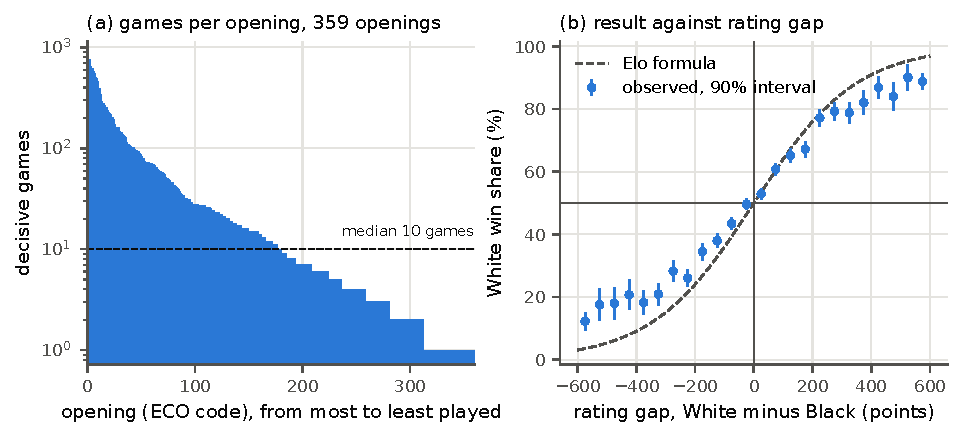
\includegraphics[width=\linewidth]{data.pdf}
  \caption{The 17,682 decisive games. (a): number of games for each of the 359 openings, identified by their ECO code, on a log scale. The data are very unbalanced: the most played opening has 821 games, the median 10, and 47 openings have a single game, which motivates a hierarchical model that pools information between openings. (b): share of games won by White in bins of 50 rating points, with 90\% binomial intervals; gaps beyond $\pm$600 points are pooled in the end bins. The dashed line is the expected score of the Elo formula, $1/(1 + 10^{-\text{gap}/400})$. The rating gap is the main driver of the result, but the observed curve is flatter than the Elo formula, so the slope $\beta$ is left free in the model. White wins more than half of the games between players of nearly equal rating (51.8\% of the 2,683 games with a gap under 25 points), which the model attributes to the first move and to the opening.}
  \label{fig:data}
\end{figure}
